\subsubsection{\stid{1.13} Argobots: Flexible, High-Performance Lightweight Threading }

\paragraph{Overview}

Efficiently supporting massive on-node parallelism demands highly
flexible and lightweight threading and tasking runtimes. At the
same time, existing lightweight abstractions have shortcomings while
delivering generality and specialization.  Our group at Argonne
developed a lightweight, low-level threading and tasking framework,
called Argobots.  The key focus areas of this project are: (1) To
provide a framework that offers powerful capabilities for users to
allow efficient translation of high-level abstractions to low-level
implementations. (2) To provide interoperability with other
programming systems such as OpenMP and MPI as well as with other
co-located I/O services. (3) To provide a programming framework that
manages hardware resources more efficiently and reduce interference
with co-located applications.

\paragraph{Key Challenges}

Several user-level threading and tasking models have been proposed in
past to address the shortcomings of OS-level threads, primarily with
respect to cost and flexibility. Their lightweight nature and flexible
generic interface play an important role at managing efficiently the
massive concurrency expected at the Exascale level.  Existing
user-level threading and tasking models, however, are either too
specific to applications or architectures or are not as powerful or
flexible. Existing runtimes tailored for generic use \cite{GNUPth,
  PLDI97_Taura, COSET05_Thibault, COB14_Nakashima, MTAAP08_Wheeler,
  PPoPP99_Taura, SenSys06_Dunkels, TBB1, EuroPar08_Perache} are
suitable as common frameworks to facilitate portability and
interoperability but offer insufficient flexibility to efficiently
capture higher-level abstractions, while specialized runtimes
\cite{ATC02_Adya, SolarisThreads, SOSP03_von_Behren, StateThreads,
  PLDI07_Li, MTAAP09_Porterfield, WMPP05_Cuvillo, IntelOMP, Nanos++,
  LCPC96_Kale, PACT14_Treichler} are oriented to a specific
environment.

\paragraph{Solution Strategy}

Argobots offers a carefully designed execution model that balances
generality of functionality with providing a rich set of controls to
allow specialization by end users or high-level programming models.
Argobots honors this high degree of expressibility through three key
aspects:

\begin{enumerate}

\item Argobots distinguishes between the requirements of different
  \emph{work units}, which are the most basic manageable
  entities. Work units that require private stacks and context-saving
  capabilities, referred to as \textit{user-level threads} (ULTs, also
  called \textit{coroutines} or \textit{fibers}), are fully fledged
  threads usable in any context.  \emph{Tasklets} do not require
  private stacks. They are more lightweight than ULTs because they do
  not incur context saving and stack management overheads.  Tasklets,
  however, are restrictive; they can be executed only as atomic work
  units that run to completion without context switching.

\item Work units execute within OS-level threads, which we refer to as
  \emph{execution streams} (ESs). Unlike existing generic runtimes,
  ESs are exposed to and manageable by users.

\item Argobots allows full control over \emph{work unit
  management}. Users can freely manage scheduling and mapping of work
  units to ESs and achieve the desired behavior.

\end{enumerate}

In order to ensure fast critical paths despite the rich set of
capabilities, Argobots was designed in a modular way to offer
configuration knobs and a rich API that allow users to trim
unnecessary costs.

\paragraph{Recent Progress}

The proposed lightweight, low-level threading and tasking framework
that is designed as a portable and performant substrate for high-level
programming models or runtime systems is called as Argobots. The
design of the Argobots is as follows:

\begin{enumerate}

\item \textbf{Execution Model:} Figure~\ref{fig:sollve-argobots}
  illustrates the execution model of Argobots. Two levels of
  parallelism are supported: ESs and work units. An ES maps to one OS
  thread, is explicitly created by the user, and executes
  independently of other ESs. A work unit is a lightweight execution
  unit, a ULT or a tasklet, that runs within an ES.  There is no
  parallel execution of work units within a single ES, but work units
  across ESs can be executed in parallel.  Each ES is associated with
  its own scheduler that is in charge of scheduling work units
  according to its scheduling policy.

\item \textbf{Scheduler:} Argobots provides an infrastructure for
  stackable or nested schedulers, with pluggable scheduling policies,
  while exploiting the cooperative non-preemptive activation of work
  units. Localized scheduling policies such as those used in current
  runtime systems, while efficient for short execution, are unaware of
  global policies and priorities. Argobots allows each ES to have its
  own schedulers.  To execute work units, an ES has at least one main
  scheduler ($S_{M}$).  A scheduler is associated with one or more
  \textit{pools} where ready ULTs and tasklets are waiting for their
  execution.  Stacking schedulers is achieved through pushing
  schedulers into a pool. When a higher-level scheduler pops a
  scheduler from its pool, the new scheduler starts its execution
  (i.e., scheduling).  Once it completes the scheduling, control
  returns to the scheduler that started the execution. To give control
  back to the parent scheduler, a scheduler can also yield.  To
  support plugging in different scheduling policies, all schedulers,
  including the main scheduler, and pools are replaceable by
  user-provided alternatives.

\item \textbf{Primitive Operations:} Argobots defines primitive
  operations for work units such as \textbf{Creation}, \textbf{Join},
  \textbf{Yield}, \textbf{Yield\_to}, \textbf{Migration} and
  \textbf{Synchronizations}. Since tasklets are used for atomic work
  without suspending, most operations presented here---except
  creation, join, and migration---apply only to ULTs.

\end{enumerate}

Argobots is implemented in C language.  An ES is mapped to a Pthread
and can be bound to a hardware processing element (e.g., CPU core or
hardware thread).  Context switching between ULTs can be achieved
through various methods, such as \texttt{ucontext},
\texttt{setjmp}/\texttt{longjmp} with
\texttt{sigaltstack}~\cite{ATC00_Engelschall}, or Boost library's
\texttt{fcontext}~\cite{fcontext}. A pool is a container data
structure that can hold a set of work units and provides operations
for insertion and deletion. Argobots relies on cooperative scheduling
of ULTs to improve resource utilization. That is, a ULT may
voluntarily yield control when idle in order to allow the underlying
ES to make progress on other work units.

\begin{figure}[htb]
  \centering
  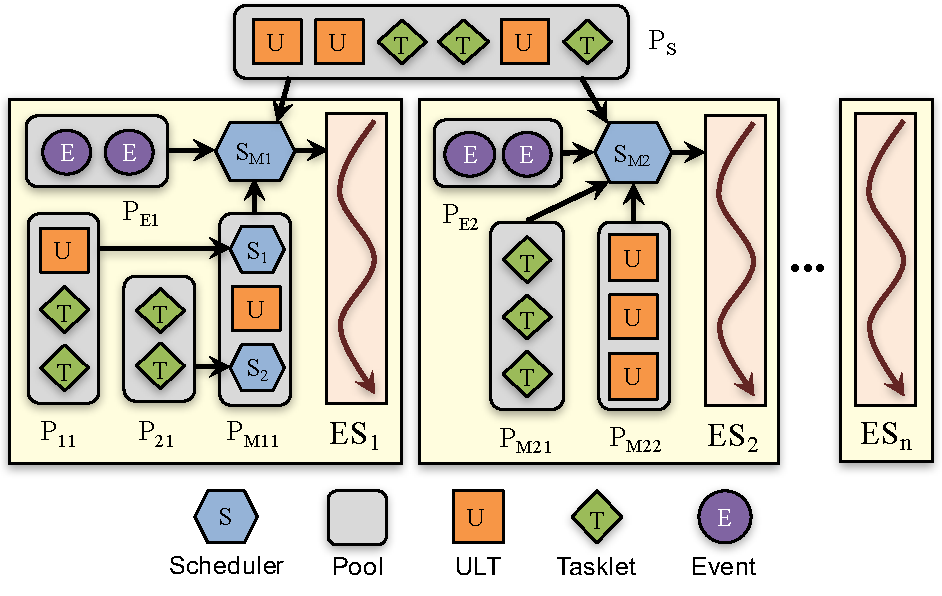
\includegraphics[height=3in]{projects/2.3.1-PMR/2.3.1.13-SOLLVE/SOLLVE-ARGOBOTS.pdf}
  \caption{\label{fig:sollve-argobots}Argobots execution model}
\end{figure}

\paragraph{Next Steps}

We studied three use cases of Argobots for higher level runtimes as
follows:

\begin{enumerate}

\item \textbf{OpenMP over Argobots:} Our OpenMP runtime implemented
  over Argobots (called BOLT) outperforms other OpenMP implementations
  because of using lightweight work units. We plan to leverage the
  supported features.

\item \textbf{Interoperability with MPI:} We investigated an MPI
  runtime that interoperates with Argobots ULTs instead of OS-level
  threads. The runtime has been shown to be subject to lock management
  issues directing us to further work on lock implementation.

\item \textbf{Colocated I/O services:} The most straightforward way to
  utilize Argobots within an I/O service daemon is to create a new ULT
  to service each incoming I/O request.  We implemented two small
  extension libraries to help support this use case.  The first,
  \emph{abt-io} and the second is \emph{abt-snoozer}. Further the
  service routines are decomposed into smaller discrete event-driven
  routines with disjoint stacks, a technique known as \emph{stack
    ripping}~\cite{ATC02_Adya}.  Presently, Argobots significantly
  reduce the development, debugging, and maintenance burden for system
  services and needs further investigations.

\end{enumerate}
